%Постановка задачи
\newpage
\chapter{ПОСТАНОВКА ЗАДАЧИ}

\subsection*{Контактные силы в классической механике}
Согласно классической механике, когда к твердому телу применяется сила, центр масс тела
в соответствии со вторым законом Ньютона, начнет двигаться в направлении вектора
единицы силы с ускорением, равным отношению величины силы и массы тела.
Поскольку реальные тела не являются абсолютно жесткими, предположение, что все тело
будет двигаться с этим ускорением конечно неверно. В действительности приложенная
сила будет инициировать волны двигающиеся по телу, которые в конечном итоге приведут
к движению всего тела. Следовательно, важным вопросом является понимание перехода от
волновых процессов к движению объекта на макроуровне

Другой важный вопрос это разница/взаимосвязь между кинетической энергией волн,
распространяющихся внутри тела, и тепловой энергией тела, и переход от одного к другому.
Силы можно условно разделить на первичные и вторичные:

\begin{itemize}
\item \textbf{Первичные силы} - являются фундаментальной характеристикой материи и представляют собой силу
соответствующего потенциального энергетического поля, к которому они принадлежат.
В классической механике Ньютона мы как правило имеем дело с гравитационными и
электромагнитными силами. Действие сил всегда осуществляется посредством полей,
создаваемых телами и воспринимаемых рассматриваемым телом.
\item \textbf{Вторичные силы} - являются результатом взаимодействия вещества, поскольку для
возникновения требуют существования контакта между объектами, то есть являются
силами второго порядка.
\end{itemize}
В соответствии с третьим законом Ньютона действие одной силы способствует появлению
равной по модулю, но противоположной по направлению силы - пара сил.
При взаимодействии двух макроскопических объектов их атомы меняют свое положение
под действием соответствующих электромагнитных силовых полей, что в макромасштабе
наблюдается как деформации взаимодействующих объектов, что может быть постоянным
процессом, периодическим или их комбинацией.
Остающийся вопрос - как такое взаимодействие между двумя объектами может быть
обеспечено?

Контактные силы можно разделить на статические и динамические:
\begin{itemize}
\item \textbf{cтатические} - обусловленные первичными силами,
\item \textbf{динамические} - образованные в процессе включающем движение материи (динамический способ
генерации контактной силы / пары сил).
\end{itemize}

Взаимодействие двух тел, как было сказано выше, инициирует волны материи на микроуровне, 
которые в дальнейшем инициируют движение на макроуровне, то возникает вопрос, какая часть энергии, запасенной телом перейдет в 
поступательную кинетическую энергию тела? Аналогом такого взаимодействия может быть любое не абсолютно упругое взаимодействие 
двух тел, при котором часть энергии взаимодействия переходят во внутреннюю энергию тела, 
то есть в тепловую. Демпфирующие полидисперсные материалы так же являются аналогом такой системы и для демпфера важно 
эффективное преобразование кинетической энергии во внутреннюю энергию системы\cite{InfluenceOfNodes}.

Поведение гранулированных материалов может проходить через различные фазы, иметь
хаотичный характер, поэтому создание общей теории, описывающее поведение
гранулированных материалов, является затруднительным. При этом такие материалы могут поглощать
приложенную энергию колебаний, а ввиду возможности создания демпфирующих
элементов из прочных материалов с небольшим весом, они нашли применение в
высокотехнологичных отраслях: в работе \cite{work1} приводится пример применения
демпфирующих элементов, основанных на гранулированных материалах, в
аэрокосмической отрасли.

В данной работе также указано на тот факт, что при низких амплитудах вибрации, когда
частицы материала постоянно находятся в контакте, эффект демпфирования будет зависеть
от способности отдельных частиц к диссипации энергии. То есть можно анализировать
поведение материала под нагрузкой на основе анализа взаимодействия его отдельных
частиц.

Работа \cite{work1} также ссылается на аналитический метод, позволяющий найти эффективный
модуль упругости и эффективное отношение Пуассона случайной упаковки для одинаковых
упругих сфер, когда они находятся в постоянном контакте (аналог низкоамплитудной
вибрации), где постоянные сжимающие силы между любыми контактирующими
частицами могут быть вызваны гидростатическим сжатием вещества.

В научной литературе принято связывать процесс диссипации с переносом энергии
вещества из различных форм в тепловую.При этом возможны процессы, также потребляющие энергию, при действии которых
тепловая энергия незамкнутой системы будет меняться незначительно. Разумеется, в
конечном итоге энергия будет переходить в тепловую, но если ограничить
рассматриваемую область областью без диссипационных процессов, то можно
рассматривать диссипацию или поглощение энергии системой, не обусловленную
процессами трения и не связанные с выделением тепла.
Данная работа основана в большой степени на гипотезе Игоря Эмри, о том что
источниками диссипации энергии в определенных системах могут выступать контактные
силы, вследствии чего потребляемая системой энергия уходит не полностью в тепло, а
частично на создание силовой сети, засчет перераспределения волновой энергии взаимодействия тел. Данная гипотеза основана на экспериментах \cite{work2, work7} с
гранулированными материалами. 

С помощью экспериментальной установки \cite{work2} позволяющей исследовать поведение
материалов под давлением, как описано в работах \cite{work2, work7} было установлено что в
определенных условиях материал (полимерное вещество под давлением), поглощающий
энергию, изменяет свою температуру незначительно, т.е. не вся переданная веществу
энергия перешла в тепло в этом веществе. Этот эффект, как оказалось, практически не
исследован в литературе.

Среди исследований данной тематике можно привести работу \cite{work10} в которой с помощью
метода конечных элементов исследуются свойства гранулированных материалов
находящихся под нагрузкой. Результаты полученные численно для определенных
параметров системы не являются универсальными, следовательно не являются
достаточным результатом для анализа процессов поглощения энергии в демпфирующем
элементе.

Похожее исследование \cite{work11} изучает динамическое поведение механической системы с
одной степенью свободы содержащей демпфер частиц.
Результаты работы демонстрируют регулярное или хаотическое движение
гранулированного слоя при частоте возбуждения в качестве параметра управления.
Результаты демонстрируют поведение слоя вещества, но элементы трения в модели не
дают изучить требуемый эффект нетепловой диссипации.
Взаимосвязь диссипации энергии и образования пары сил или силовой сети в
гранулированных системах не изучена, а поскольку процессы диссипации могут иметь
практическое применение, было решено исследовать процесс, обуславливающий работу
демпфирующего элемента, то есть процесс диссипации энергии в гранулированных
материала.

Так же был произведен эксперимент, в котором по пластине из полидисперсного полимера заданной ширины стреляют пулей со скоростью 45 м/с, что приводит в разрушению пластины. Затем такой же пулей, с той же скоростью стреляют по пластине из того же полимера, но теперь ширина пластины уменьшена в два раза. 
В результате взаимодействия полимер не только не разрушается, но и останавливает пулю, что говорит о скрытых процессах внутри материала и влиянии процесса создания силовой сети на распространение деформаций и диссипацию энергии в материалах.

Таким образом для понимания процессов, происходящих в гранулированных материалах было решено проанализировать многоуровневый энергетический обмен в простейшей силовой сети и ее образования. Данный процесс рассматривается на двух различных уровнях: на внешнем - макроуровне(рисунок \ref{fig:micmac} (а) ), и на внутреннем - микроуровне(рисунок \ref{fig:micmac} (б) ). 

Простейшим примером взаимодействия на макроуровне является столкновение эластичного сферического тела массой $M$, которое движется с постоянной скоростью $v_0$, с жесткой стенкой. В процессе взаимодействия, согласно третьему закону Ньютона, между телом и жесткой стенкой сформируется пара сил: тело будет давить на стенку с силой $F$, а стенка будет давить на тело с силой $-F$. Последняя сила, в свою очередь, в течении времени $\Delta t$ остановит тело и ускорит его в обратном направлении со скоростью $-v_0$. Во время соударения внешняя кинетическая энергия будет превращена во внутреннюю потенциальную энергию эластичного тела. При этом многоуровневом взаимодействии и преобразовании энергии формируется контактная пара сил. Таким образом контактные силы являются результатом многоуровневого преобразования энергий.

Рассмотрим данный процесс на микроуровне. Представим тело в качестве системы нескольких тел с массами $m_1$, $m_2$, $m_3$, соединенных пружинами с жесткостями $k_2$, $k_3$, тогда внутренняя энергия системы будет заключена в кинетической энергии относительного движения частиц и энергии пружин. При этом взаимодействие тела с жесткой стенкой происходит посредством пружины жесткостью $k_1$. Преобразование энергий заключается в переходе внешней кинетической энергии движения масс, во внутреннюю энергию, аналогом которой в данной постановке задачи являются потенциальные энергии пружин, соединяющих массы, и кинетические энергии относительного движения масс. Таким образом, найдя энергию поступательного движения тела после соударения, мы можем узнать диссипацию энергии в системе, что не позволяет сделать анализ на макроуровне.

\begin{figure}[h]
    \begin{minipage}[h]{0.3\linewidth}
    \center{
        

\tikzset{every picture/.style={line width=0.75pt}} %set default line width to 0.75pt        

\begin{tikzpicture}[x=0.75pt,y=0.75pt,yscale=-1,xscale=1]
%uncomment if require: \path (0,244.3173065185547); %set diagram left start at 0, and has height of 244.3173065185547

%Straight Lines [id:da41391987557326315] 
\draw    (50.43,48.24) -- (50.43,234.24) ;


%Straight Lines [id:da8975629204988387] 
\draw    (50.43,70.24) -- (39.77,60.16) ;
\draw    (49.77,90.24) -- (39.1,80.16) ;
\draw    (50.43,110.24) -- (39.77,100.16) ;
\draw    (50.43,130.91) -- (39.77,120.83) ;


%Straight Lines [id:da3207421376516373] 
\draw    (51.1,150.91) -- (40.43,140.83) ;


%Straight Lines [id:da4433189705331644] 
\draw    (51.1,170.91) -- (40.43,160.83) ;


%Straight Lines [id:da1320019866862019] 
\draw    (50.43,191.58) -- (39.77,181.5) ;


%Straight Lines [id:da17396697635412584] 
\draw    (50.43,210.91) -- (39.77,200.83) ;


%Straight Lines [id:da7024410341299809] 
\draw    (49.77,228.91) -- (39.1,218.83) ;


%Shape: Circle [id:dp7508815890818632] 
\draw   (100,139) .. controls (100,125.19) and (111.19,114) .. (125,114) .. controls (138.81,114) and (150,125.19) .. (150,139) .. controls (150,152.81) and (138.81,164) .. (125,164) .. controls (111.19,164) and (100,152.81) .. (100,139) -- cycle ;
%Straight Lines [id:da41402643933373806] 
\draw    (114.31,102.16) -- (135.97,102.16) ;

\draw [shift={(112.31,102.16)}, rotate = 0] [fill={rgb, 255:red, 0; green, 0; blue, 0 }  ][line width=0.75]  [draw opacity=0] (8.93,-4.29) -- (0,0) -- (8.93,4.29) -- cycle    ;

% Text Node
\draw (126.67,86.67) node  [align=left] {$\displaystyle v_0$};
% Text Node
\draw (125,139) node  [align=left] {$\displaystyle M$};


\end{tikzpicture} \\ а)
    }
    \end{minipage}
    \hfill  
    \begin{minipage}[h]{0.3\linewidth}
    \center{
         

\tikzset{every picture/.style={line width=0.75pt}} %set default line width to 0.75pt        

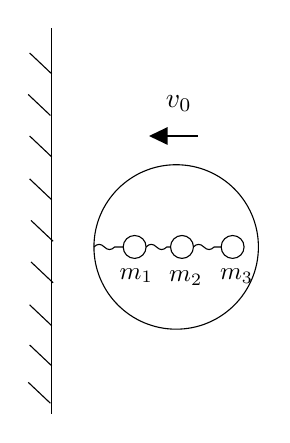
\begin{tikzpicture}[x=0.75pt,y=0.75pt,yscale=-1,xscale=1]
%uncomment if require: \path (0,244.3173065185547); %set diagram left start at 0, and has height of 244.3173065185547

%Straight Lines [id:da41391987557326315] 
\draw    (50.43,48.24) -- (50.43,234.24) ;


%Straight Lines [id:da8975629204988387] 
\draw    (50.43,70.24) -- (39.77,60.16) ;


%Straight Lines [id:da4791030925335944] 
\draw    (49.77,90.24) -- (39.1,80.16) ;


%Straight Lines [id:da9564038647659947] 
\draw    (50.43,110.24) -- (39.77,100.16) ;


%Straight Lines [id:da6270302864150106] 
\draw    (50.43,130.91) -- (39.77,120.83) ;


%Straight Lines [id:da3207421376516373] 
\draw    (51.1,150.91) -- (40.43,140.83) ;


%Straight Lines [id:da4433189705331644] 
\draw    (51.1,170.91) -- (40.43,160.83) ;


%Straight Lines [id:da1320019866862019] 
\draw    (50.43,191.58) -- (39.77,181.5) ;


%Straight Lines [id:da17396697635412584] 
\draw    (50.43,210.91) -- (39.77,200.83) ;


%Straight Lines [id:da7024410341299809] 
\draw    (49.77,228.91) -- (39.1,218.83) ;


%Shape: Circle [id:dp7508815890818632] 
\draw   (70.76,153.62) .. controls (70.76,131.74) and (88.5,114) .. (110.38,114) .. controls (132.26,114) and (150,131.74) .. (150,153.62) .. controls (150,175.5) and (132.26,193.24) .. (110.38,193.24) .. controls (88.5,193.24) and (70.76,175.5) .. (70.76,153.62) -- cycle ;
%Straight Lines [id:da41402643933373806] 
\draw    (99.31,100.16) -- (120.97,100.16) ;

\draw [shift={(97.31,100.16)}, rotate = 0] [fill={rgb, 255:red, 0; green, 0; blue, 0 }  ][line width=0.75]  [draw opacity=0] (8.93,-4.29) -- (0,0) -- (8.93,4.29) -- cycle    ;
%Shape: Circle [id:dp6894624139524745] 
\draw   (84.85,153.62) .. controls (84.85,150.57) and (87.32,148.1) .. (90.37,148.1) .. controls (93.42,148.1) and (95.89,150.57) .. (95.89,153.62) .. controls (95.89,156.67) and (93.42,159.14) .. (90.37,159.14) .. controls (87.32,159.14) and (84.85,156.67) .. (84.85,153.62) -- cycle ;
%Shape: Circle [id:dp7196151672559912] 
\draw   (107.66,153.62) .. controls (107.66,150.57) and (110.13,148.1) .. (113.18,148.1) .. controls (116.23,148.1) and (118.7,150.57) .. (118.7,153.62) .. controls (118.7,156.67) and (116.23,159.14) .. (113.18,159.14) .. controls (110.13,159.14) and (107.66,156.67) .. (107.66,153.62) -- cycle ;
%Shape: Circle [id:dp6290232420684407] 
\draw   (132.06,153.62) .. controls (132.06,150.57) and (134.53,148.1) .. (137.58,148.1) .. controls (140.63,148.1) and (143.1,150.57) .. (143.1,153.62) .. controls (143.1,156.67) and (140.63,159.14) .. (137.58,159.14) .. controls (134.53,159.14) and (132.06,156.67) .. (132.06,153.62) -- cycle ;
%Straight Lines [id:da4539197689910155] 
\draw    (70.76,153.62) .. controls (72.43,151.95) and (74.09,151.95) .. (75.76,153.62) .. controls (77.43,155.29) and (79.09,155.29) .. (80.76,153.62) -- (84.85,153.62) -- (84.85,153.62) ;


%Straight Lines [id:da14488596850940327] 
\draw    (95.89,153.62) .. controls (97.56,151.95) and (99.22,151.95) .. (100.89,153.62) .. controls (102.56,155.29) and (104.22,155.29) .. (105.89,153.62) -- (107.66,153.62) -- (107.66,153.62) ;


%Straight Lines [id:da4969696424254402] 
\draw    (118.7,153.62) .. controls (120.37,151.95) and (122.03,151.95) .. (123.7,153.62) .. controls (125.37,155.29) and (127.03,155.29) .. (128.7,153.62) -- (132.06,153.62) -- (132.06,153.62) ;



% Text Node
\draw (111.67,84.67) node  [align=left] {$\displaystyle v_{0}$};
% Text Node
\draw (84.87,170.12) node [scale=0.5] [align=left] {$ $};
% Text Node
\draw (91.1,167.5) node [scale=0.9] [align=left] {$\displaystyle m_{1}$};
% Text Node
\draw (115,168.5) node [scale=0.9] [align=left] {$\displaystyle m_{2}$};
% Text Node
\draw (139.5,167.8) node [scale=0.9] [align=left] {$\displaystyle m_{3}$};


\end{tikzpicture}
 \\ б)
    }
    \end{minipage}
    \caption{Модель тела из полидисперсного материала на макроуровне (а) и на микроуровне (б)}
    \label{fig:micmac}
\end{figure}


%\begin{figure}[h]
%    \centering
%    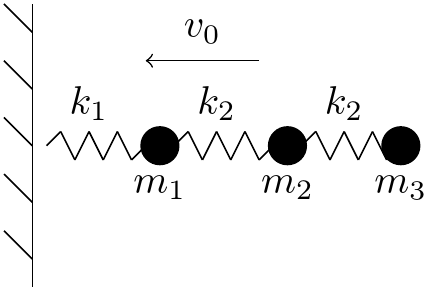
\includegraphics[width=0.4\textwidth]{sketch.png}
%    \caption{Эскиз системы трех тел. Все тела разделены пружинами длины $l$.}
%    \label{fig:sketch}
%\end{figure}

